\section{Introduction}
\label{sec:01:intro}

\renewcommand{\currprop}{0.8\textwidth}

\begin{frame}{Motivation: From the Green to a ``Greener Revolution''}
    \begin{block}{The Green Revolution (1960s-70s)}
        \begin{itemize}
            \item \textbf{Success:} Led to a giant increase in agricultural production.
            \item \textbf{Drawbacks \& Legacy:} Established widespread monocultures and advanced machinery, but introduced severe environmental impacts (deforestation, pollution, and biodiversity loss).
        \end{itemize}
    \end{block}
    
    \pause
    
    \begin{block}{The Current Challenge (A ``Greener Revolution'')}
        \begin{itemize}
            \item \textbf{The Need:} As the global population continues to grow, a further leap in agricultural productivity is required.
            \item \textbf{The Challenge:} This new leap must be strictly sustainable, mitigating the agribusiness environmental footprint and addressing current climate problems.
        \end{itemize}
    \end{block}
\end{frame}

\begin{frame}{The Tool: Remote Sensing (RS)}
    \renewcommand{\currprop}{0.5\textheight}
    \begin{block}{Definition}
        RS is the technology of collecting information about Earth's surface from distance, without direct physical contact, using sensors installed on platforms such as satellites or aircraft.
    \end{block}
    \begin{figure}
        \centering
        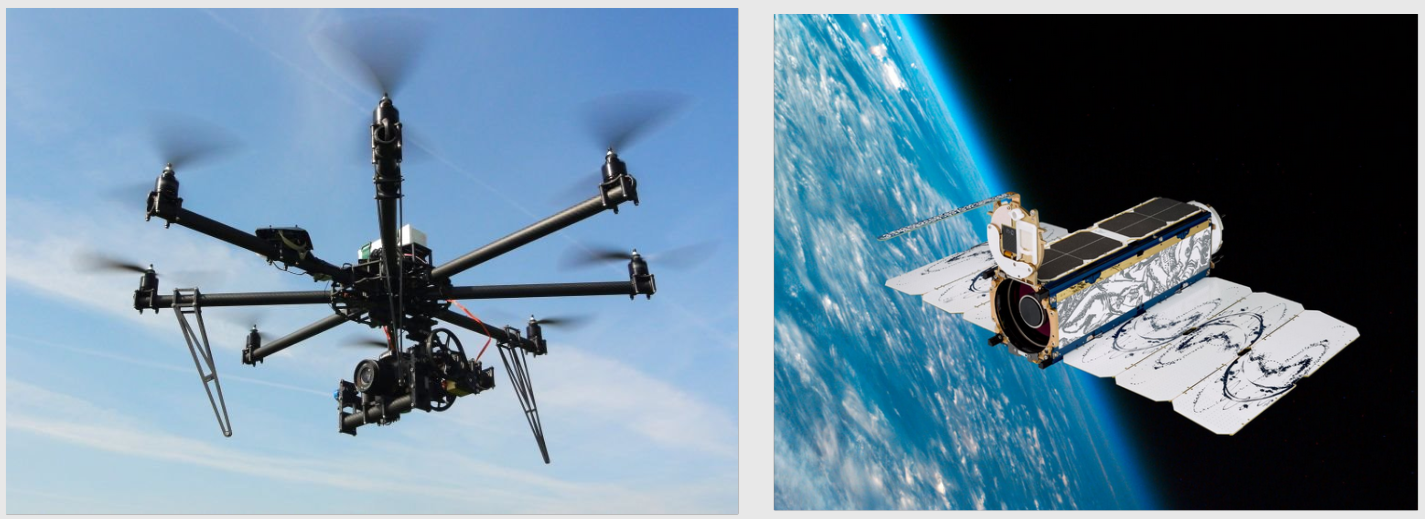
\includegraphics[height=\currprop]{figures/99_slides_only/drone_and_satellite.png}
    \end{figure}
\end{frame}

\begin{frame}{The Tool: Remote Sensing (RS)}
    \begin{block}{RS as a Key Enabler}
        In this context, Remote Sensing (RS) is a candidate tool to help accomplish this new "greener revolution".
        \begin{itemize}
            \pause
            \item It allows monitoring optimal planting and harvesting conditions.
            \pause
            \item It enables Precision Agriculture (e.g., applying chemicals locally rather than uniformly).
            \pause
            \item It allows active monitoring of deforestation.
            \pause
            \item It helps stakeholders anticipate food shortages.
        \end{itemize}
    \end{block}
\end{frame}

\begin{frame}{The Challenges}
    \begin{itemize}
        \item Expert data labeling for RS is highly expensive. Conversely, free public maps (like MapBiomas or USDA CDL) often contain noisy or inconsistent labels.
        \pause
        \item The complexity increases with the size and heterogeneity of Satellite Image Time Series (SITS).
        \pause
        \item Modern Deep Neural Networks suffer from overconfidence: they exhibit high certainty even in incorrect predictions.
    \end{itemize}
\end{frame}

\begin{frame}{The Proposed Solutions}
    \begin{itemize}
        \item Instead of just improving models, \textbf{DCAI} focuses on improving data quality. We can apply rigorous filtering to noisy public labels to create highly reliable datasets.
        \pause
        \item The amount of public RS data is massive. \textbf{SSL} extracts patterns from this unlabeled data to generate supervisory signals.
        \pause
        \item To address overconfidence, we can treat incorrect predictions as anomalies in the model's embedding space. We propose \textbf{ORDER} (Open-set Recognition for Discriminative Error Rebuttal), a post-processing strategy using Gaussian Mixture Models (GMMs) to separate correct from incorrect predictions dynamically.
    \end{itemize}
\end{frame}

\begin{frame}{Common RS Agricultural Applications}
    \renewcommand{\currprop}{0.5\textheight}
    \begin{figure}
        \centering
        \includegraphics<1| handout:0>[height=0.87\textheight]{figures/1_introduction/graphical_abstract_crop_new_fixed.pdf}
        \includegraphics<2| handout:1>[height=0.87\textheight]{figures_slides/graphical_abstract_crop_new_fixed_show.jpg}
    \end{figure}
\end{frame}

\begin{frame}{Objectives and Scope}
    \begin{block}{Objectives of This Work}
        \begin{itemize}
            \item \textbf{General Objective:} Develop and validate a reliable, lightweight, data-centric pipeline for parcel-level crop classification using SITS, capable of predicting its own failures.
            \pause
            \item \textbf{Specific Objectives:} 
            \begin{itemize}
                \item Curate public datasets using DCAI strategies.
                \item Benchmark classification architectures (from Shallow to Mamba/Transformers) and SSL techniques.
                \item Develop a confidence estimation strategy (ORDER) to rebut classification errors.
            \end{itemize}
        \end{itemize}
    \end{block}
\end{frame}

\begin{frame}{Research Questions}
    \begin{enumerate}
        \item \textbf{RQ1:} To what extent can DCAI strategies - specifically, rigorous filtering of noisy public labels (such as USDA CDL or Mapbiomas) - enable the creation of crop classification datasets and improve the performance of crop classification models?
        \item \textbf{RQ2:} Do SSL pre-training strategies impact embedding generation and offer a significant advantage over supervised models when labels are scarce? If so, which strategy generates the best embeddings?
        \item \textbf{RQ3:} Is it possible to build a lightweight pipeline that achieves satisfactory performance for crop classification that can be run without expensive hardware? If so, which models are most suitable?
    \end{enumerate}
\end{frame}

\begin{frame}{Research Questions}
    \begin{enumerate}
        \item \textbf{RQ4:} Is it possible to achieve satisfactory performance for crop classification using only public sensors?
        \item \textbf{RQ5:} Is it possible to improve confidence estimation or detect model anomalies - differ between right and wrong predictions - through generative models on embeddings, surpassing established baselines such as ConfidNet in the task of fault prediction?
    \end{enumerate}
\end{frame}